\documentclass[border=5mm]{standalone}
\usepackage{tikz}
\usepackage{amsmath}

\usetikzlibrary{arrows.meta, positioning, calc}

\begin{document}
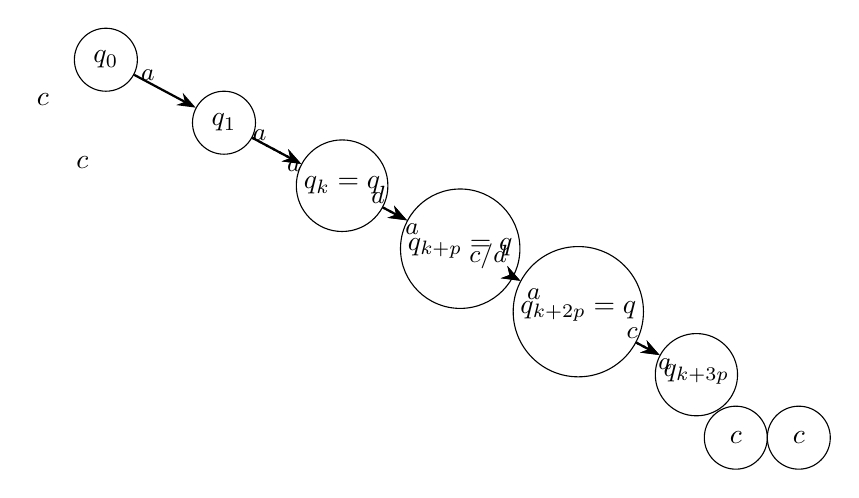
\begin{tikzpicture}[
    node distance=1.2cm and 2.5cm,
    >=Stealth,
    state/.style={
        circle,
        draw,
        minimum size=0.8cm,
        inner sep=2pt
    },
    solid edge/.style={
        ->,
        thick
    },
    dotted edge/.style={
        ->,
        dotted,
        thick
    }
]

% 状态节点
\node[state] (q0) at (0,0) {$q_0$};
\node[state] (q1) at (1.5,-0.8) {$q_1$};
\node[state] (qk) at (3,-1.6) {$q_k = q$};
\node[state] (qkp) at (4.5,-2.4) {$q_{k+p} = q$};
\node[state] (qk2p) at (6,-3.2) {$q_{k+2p} = q$};
\node[state] (qk3p) at (7.5,-4) {$q_{k+3p}$};

% 实线箭头
\draw[solid edge] (q0) -- node[midway, above left, font=\small] {$a$} (q1);
\draw[solid edge] (q1) -- node[midway, above left, font=\small] {$a$} (qk);
\draw[solid edge] (qk) -- node[midway, above left, font=\small] {$d$} (qkp);
\draw[solid edge] (qkp) -- node[midway, above left, font=\small] {$c/d$} (qk2p);
\draw[solid edge] (qk2p) -- node[midway, above left, font=\small] {$c$} (qk3p);

% 虚线箭头
\draw[dotted edge] (q1) -- node[midway, below right, font=\small] {$a$} (qk);
\draw[dotted edge] (qk) -- node[midway, below right, font=\small] {$a$} (qkp);
\draw[dotted edge] (qkp) -- node[midway, below right, font=\small] {$a$} (qk2p);
\draw[dotted edge] (qk2p) -- node[midway, below right, font=\small] {$a$} (qk3p);

% 左侧标签
\node at (-0.8,-0.5) {$c$};
\node at (-0.3,-1.3) {$c$};

% 最右侧节点
\node[state] (cqk3p1) at (8,-4.8) {$c$};
\node[state] (cqk3p2) at (8.8,-4.8) {$c$};

\end{tikzpicture}
\end{document}